\documentclass[10pt,landscape]{article}
\usepackage{multicol}
\usepackage{calc}
\usepackage{ifthen}
\usepackage[landscape]{geometry}
\usepackage[ngerman]{babel}
\usepackage[utf8]{inputenc}
\usepackage{graphics}
\usepackage{listings}
\usepackage{verbatim}


% This sets page margins to .5 inch if using letter paper, and to 1cm
% if using A4 paper. (This probably isn't strictly necessary.)
% If using another size paper, use default 1cm margins.
\ifthenelse{\lengthtest { \paperwidth = 11in}}
	{ \geometry{top=.5in,left=.3in,right=.5in,bottom=.5in} }
	{\ifthenelse{ \lengthtest{ \paperwidth = 297mm}}
		{\geometry{top=1cm,left=1cm,right=1cm,bottom=1cm} }
		{\geometry{top=1cm,left=1cm,right=1cm,bottom=1cm} }
	}

% Turn off header and footer
\pagestyle{empty}
 

% Redefine section commands to use less space
\makeatletter
\renewcommand{\section}{\@startsection{section}{1}{0mm}%
                                {-1ex plus -.5ex minus -.2ex}%
                                {0.5ex plus .2ex}%x
                                {\normalfont\large\bfseries}}
\renewcommand{\subsection}{\@startsection{subsection}{2}{0mm}%
                                {-1explus -.5ex minus -.2ex}%
                                {0.5ex plus .2ex}%
                                {\normalfont\normalsize\bfseries}}
\renewcommand{\subsubsection}{\@startsection{subsubsection}{3}{0mm}%
                                {-1ex plus -.5ex minus -.2ex}%
                                {1ex plus .2ex}%
                                {\normalfont\small\bfseries}}
% Special commands
\newcommand{\code}[1]{\texttt{#1}}

\makeatother

% Define BibTeX command
\def\BibTeX{{\rm B\kern-.05em{\sc i\kern-.025em b}\kern-.08em
    T\kern-.1667em\lower.7ex\hbox{E}\kern-.125emX}}

% Don't print section numbers
\setcounter{secnumdepth}{0}


\setlength{\parindent}{0pt}
\setlength{\parskip}{0pt plus 0.5ex}


% -----------------------------------------------------------------------

\begin{document}

\raggedright
\footnotesize
\begin{multicols}{3}


% multicol parameters
% These lengths are set only within the two main columns
%\setlength{\columnseprule}{0.25pt}
\setlength{\premulticols}{1pt}
\setlength{\postmulticols}{1pt}
\setlength{\multicolsep}{1pt}
\setlength{\columnsep}{2pt}

\begin{center}
     \Large{\textbf{Codierung CheatSheet}} \\
\end{center}

\section{Verschl"usselungsverfahren}
\subsection{Perfekt sicherer Code}
\textbf{One-Time-pad code} \\
\begin{itemize}
    \item Codierungsschl"ussel genau so lang wie der zu kodierende Text.
    \item Schl"ussel zuf"allig
    \item Kommis sind nur aufgeflogen, weil sie die Schl"ussel recycelt haben
\end{itemize}
\subsection{Was bedeutet Perfekt?}
$P(m) = P(m|C)$

\subsection{Public-Key}
Besteht aus "offentlichem und privaten Teil.\\
Der "offentliche ist wie ein offenes Schloss, der genutzt werden kann, um etwas nur mit dem privaten Schl"ussel zugreifbar zu machen.

\subsubsection{RSA}
Basiert drauf das die Primzahlfaktorisierung NP-vollst"andig ist.
\paragraph{Erzeugung RSA-Code} \ \\
\begin{itemize}
    \item bestimme p,q die Primzahlen sind und weit genug auseinanderliegen
    \item dann $n = p*q$ und $\phi(n) = (p-1) (q-1) := \#$der Zahlen, die zu n teilerfremd sind.
    \item w"ahle "offentlichen Schl"ussel e mit $ggt(\phi(n), e) = 1$
    \item finde durch EEA(erweiterter Euklidischen algorithmus) ein d sodass $e*d ^= 1 (mod phi(n))$
    \item mann verschl"usselt dann mit $m^e$ und entschl"usselt mit $(m^e)^d$
\end{itemize}

\paragraph{Warum klappt codierung/decod.?} \ \\
$ed= 1(mod phi(n))$

\paragraph{Und wie genau?} \ \\
$ed = 1 + k * phi(n)$\\
$m ^(1 + k * phi(n))$\\
$m * m^(k * phi(n))$\\
$m * (m^(p-1))^(k* (q-1))$\\
$m * 1, da Fermatsatz: m^(p-1) = 1 (mod p) -> = 1 (mod p * q)$
\subsubsection{Wie funktioniert dann El-Gamal?}
$(p,g, g^a)$ "offentlich, $a$ geheim \\
jemand w"ahlt $b$ (geheim) und sendet $(g^b, m * g^ab)$ \\
Empf"anger macht dann $(g^ba)^-1$ und kann so entschl"usseln
\subsubsection{Deffie Halman}
Alice w"ahlt a und sendet A,g,p $A = g^a mod p$. Bob sendet $B = g^b mod p$.\\
Nun kann jeder der beiden ein K bilden mit $K = A^b mod p$ bzw. $K = B^a mod p$.
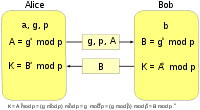
\includegraphics{200px-Diffie-Hellman-Schluesselaustausch.png}

\subsection{Warum sind die sicher, wenn $NP!=P$?}
\begin{itemize}
    \item RSA weil Primzahlzerlegung NP-vollst"andig
    \item El-Gamal weil es keinen diskreten Algo gibt
\end{itemize}
\subsection{Und wenn $NP=P$...}
\textbf{Weltuntergang!} \\
Bei NP kann man raten und dann in poly. berechnen, dauert halt ewig, weil man nur raten kann.\\
Wenn man jedoch nicht mehr raten muss, sondern z.B. Primfaktoren in poly. berechnen k"onnte, dann w"urde das Kartenhaus zusammenfallen.\\
Auf $NP!=P$ basiert unsere Sicherheit.

\subsection{Was ist sicherer (RSA oder El Gamal)?}
El Gamal, da sich der Schl"ussel "andert.

\subsubsection{Hat El Gamal auch Nachteile?}
\begin{itemize}
    \item \textbf{Hauptnachteil} ist, dass es sichere Zufallszahlen braucht
    \item Ausserdem wird der verschl"usselte Text doppelt so gross wie das Original (?)
\end{itemize}

\subsubsection{Gegen was ist ElGamal immun, das RSA belastet?}
W"orterbuchangriffe, da sich der Schl"ussel bei RSA nicht "andert,  kann er leichter erraten werden.

\subsubsection{Welche Angriffe gibt es noch?}
\begin{itemize}
    \item known plaintext
    \item known chiffretext
    \item chosen plaintext
    \item chosen chiffretext
    \item man-in-the-middle
\end{itemize}


\subsubsection{Was ist ein Geburtstagsangriff}
Kommt bei Hashwerten zum Einsatz, man suucht nach zwei gleichen Hashwerten.
Formel zur Berechnung wie viele W"orter man braucht: $1.18*\sqrt{m}$

\subsubsection{Man-In-The-Middle}
Jemand schaltet sich in die Mitte

\subsection{Hamming-Code}
\subsubsection{Kugelpackungsschranke}
$|C| \leq \frac{q^n}{\sum^t_{i=0}{{n \choose i} (q-1)^i}}$ \\
$n = Codel"ange$ \\ 
$q = Alphabetm"achtigkeit$ \\
$t = Radius der Kugel$\\
\subsubsection{Decodierung HC}
Codewort wird Kugel mit geringster Hammingdistanz zugeordnet.

\subsubsection{Linearer Code}
Codewortraum ist K"orper und untervektorraum von V.
\paragraph{Wie viele Fehler k"onnen korrigiert werden?}
$maximal (d(C)-1)/2$ \\
\paragraph{Syndrome} 
Alle Elemente einer Nebenklasse haben das gleiche Syndrom. \\
Wird nun ein Codewort "ubermittelt, dann kann anhand des Syndroms ermittelt werden, zu welcher Nebenklasse es geh"ort. \\
Der Nebenklassenf"uhrer (geringster Hammingabstand zum Nullvektor) gibt an, welche Bits fehlerhaft sind.

\subsection{Reed-Solomon}
Kommt bei der Audio-CD, DVB,DAB und bei der Kommunikation mit Raumsonden.
\subsubsection{Interleaving}
Beim Interleaving werden die Codew"orter spaltenweise geschrieben und zeilenweise gelesen. \\
Dadurch verliert man nicht h"appchenweise Information.
\subsubsection{Cross Interleaving}
Die Codew"orter werden "ueber drei Puffer verz"ogert verarbeitet, dadurch erh"ote Streuung und mehr Fehlertoleranz.

\subsection{Primzahltests}
\subsubsection{Fermat-Test}
Geht flink, f"allt jedoch auf Charlmichael-Zahlen herein. Macht nur eine kontraproduktive Aussage.
Wenn er sagt ist keine, dann isses auch keine. Wenn er sagt iss eine, dann evtl. Charlmichael.

\subsubsection{Miller Rabin}
Gibt nur bestimmte Wahrscheinlichkeit ab. Normalerweise, m"ussten alle Zeugen befragt werden, sind jedoch nen ganzer Haufen.
Daher setzt man sich eine Wahrscheinlichkeit und ist dann zufrieden.

\end{multicols}
\end{document}
